%file main.tex
%Adapted from
%http://yetanotherbiochemblog.wordpress.com/2011/10/11/managing-conference-materials-in-latex-part-1-abstract-template/
%Edited vss APRIL/2012

\documentclass[11pt,a5paper,twoside]{book}
\usepackage[a5paper]{geometry}
\usepackage[utf8x]{inputenc}
\usepackage[T1]{fontenc}
\usepackage[english]{babel}
\usepackage{fixltx2e}
\usepackage{hyphenat}
\usepackage[usenames,dvipsnames]{color}
%\usepackage{multicols}
\usepackage{longtable}
%\usepackage{marvosym}



%a5 paper= 	148mm x 210mm
%a4 paper=	210mm x 297mm
\setlength\hoffset{-0.79cm} % 1
\setlength\oddsidemargin{0cm} % 3
\setlength\evensidemargin{0cm} % 3
\setlength\textwidth{110mm} % 8
\setlength\voffset{-2.54cm} % 2
\setlength\topmargin{1.1cm} % 4
\setlength\headheight{0.7cm} % 5
\setlength\headsep{0.4cm} % 6
\setlength\textheight{170mm} % 7
%\setlength\footskip{1.0cm} % 11
\parindent=0cm
\parskip=0.1cm

\renewcommand{\rmdefault}{ptm}

\newcommand{\anumber}[1]{\leavevmode{\textbf{#1}}}
\newcommand{\atitle}[1]{\leavevmode{\textbf{\large #1}}}
\newcommand{\affiliation}[1]{\leavevmode{\textit{#1}}}
\newcommand{\email}[1]{\leavevmode{\url{#1}}}
\newcommand{\presenting}[1]{\leavevmode{\textbf{\underline{#1}}}}
\newcommand{\authors}[1]{\textbf{\small #1}}

\usepackage{graphicx}
\usepackage{wrapfig}
\newcommand{\photo}[1]{
    \begin{wrapfigure}[4]{o}{0.2\textwidth}
    \includegraphics[width=0.2\textwidth]{#1}
    \end{wrapfigure}
}

\usepackage{fancyhdr}
\renewcommand{\headrulewidth}{0.2pt}
\renewcommand{\footrulewidth}{0.2pt}

\newcommand{\redefineheaders}[2]{
    \pagestyle{fancy}
    \fancyhf{}
    \fancyhead[L]{}
    \fancyhead[CO,CE]{}
    \fancyhead[R]{\small #2}
    \fancyfoot[R]{\thepage}
    \fancyfoot[CO,CE]{}
    \fancyfoot[L]{\textit{GRB 2012 - May 7-11, Munich, Germany}}
}

\usepackage{enumerate}

\usepackage{makeidx}
\makeindex

\begin{document}
\title{Abstracts}
\maketitle

\redefineheaders{Monday, May 7}{Session I: Recent results from Swift and Fermi}
$ABSTRACT_SESSION_I_1

\redefineheaders{Monday, May 7}{Session IIa: Prompt Emission Spectroscopy}
$ABSTRACT_SESSION_IIa_2a

\redefineheaders{Monday, May 7}{Session IIb: Prompt Emission Spectroscopy}
$ABSTRACT_SESSION_IIb_2b

\redefineheaders{Monday, May 7}{Session IIc: Prompt Emission Correlations and Temporal Properties}
$ABSTRACT_SESSION_IIc_2c

\redefineheaders{Tuesday, May 8}{Session IId: Very High-Energy Emission}
$ABSTRACT_SESSION_IId_2d

\redefineheaders{Tuesday, May 8}{Session IIIa: Afterglow Theory}
$ABSTRACT_SESSION_IIIa_3a

\redefineheaders{Tuesday, May 8}{Session IIIb: Afterglow Observatons}
$ABSTRACT_SESSION_IIIb_3b

\redefineheaders{Tuesday, May 8}{Session IIIc: Afterglow Observations}
$ABSTRACT_SESSION_IIIc_3c

\redefineheaders{Wednesday, May 9}{Session IVa: GRBs as Probes of the Early Universe}
$ABSTRACT_SESSION_IVa_4a

\redefineheaders{Wednesday, May 9}{Session IVb: GRBs as Probes of the Early Universe}
$ABSTRACT_SESSION_IVb_4b

\redefineheaders{Thursday, May 10}{Session Va: Progenitors of Long Duration Bursts}
$ABSTRACT_SESSION_Va_5a

\redefineheaders{Thursday, May 10}{Session Vb: Progenitors of Short Duration Bursts}
$ABSTRACT_SESSION_Vb_5b

\redefineheaders{Thursday, May 10}{Session Vc: Central Engine Physics}
$ABSTRACT_SESSION_Vc_5c

\redefineheaders{Thursday, May 10}{Session VI: History and Future Instrumentation}
$ABSTRACT_SESSION_VI_6

\redefineheaders{Friday, May 11}{Session VII: Grav. Waves, Neutrinos, Cosmic Rays and UHE Emission}
$ABSTRACT_SESSION_VII_7

\redefineheaders{Friday, May 11}{Session VIII: Host Galaxies}
$ABSTRACT_SESSION_VIII_8

\newpage %Make a nice poster session cover page?

\redefineheaders{}{P-II: Prompt and High-Energy Emission}
$POSTERS_SESSION_PII_p2
\redefineheaders{}{P-III: Afterglow Emission}
$POSTERS_SESSION_PIII_p3
\redefineheaders{}{P-IV: Probes of the Early Universe}
$POSTERS_SESSION_PIV_p4
\redefineheaders{}{P-V: Progenitors and Central Engine Physics}
$POSTERS_SESSION_PV_p5
\redefineheaders{}{P-VI: History and Future Instrumentation}
$POSTERS_SESSION_PVI_p6
\redefineheaders{}{P-VII: Grav. Waves, Neutrinos, Cosmic Rays and UHE Emission}
$POSTERS_SESSION_PVII_p7
\redefineheaders{}{P-VIII: Host Galaxies}
$POSTERS_SESSION_PVIII_p8

\newpage

\redefineheaders{}{List of Participants}
\title{List of Participants}

\begin{multicols}{2}



\begin{center}
  \begin{tabular}{ l | c || r | }
    \hline
$LOP
    \hline
  \end{tabular}
\end{center}

\end{multicols}


\newpage

\redefineheaders{}{Poster Guide}

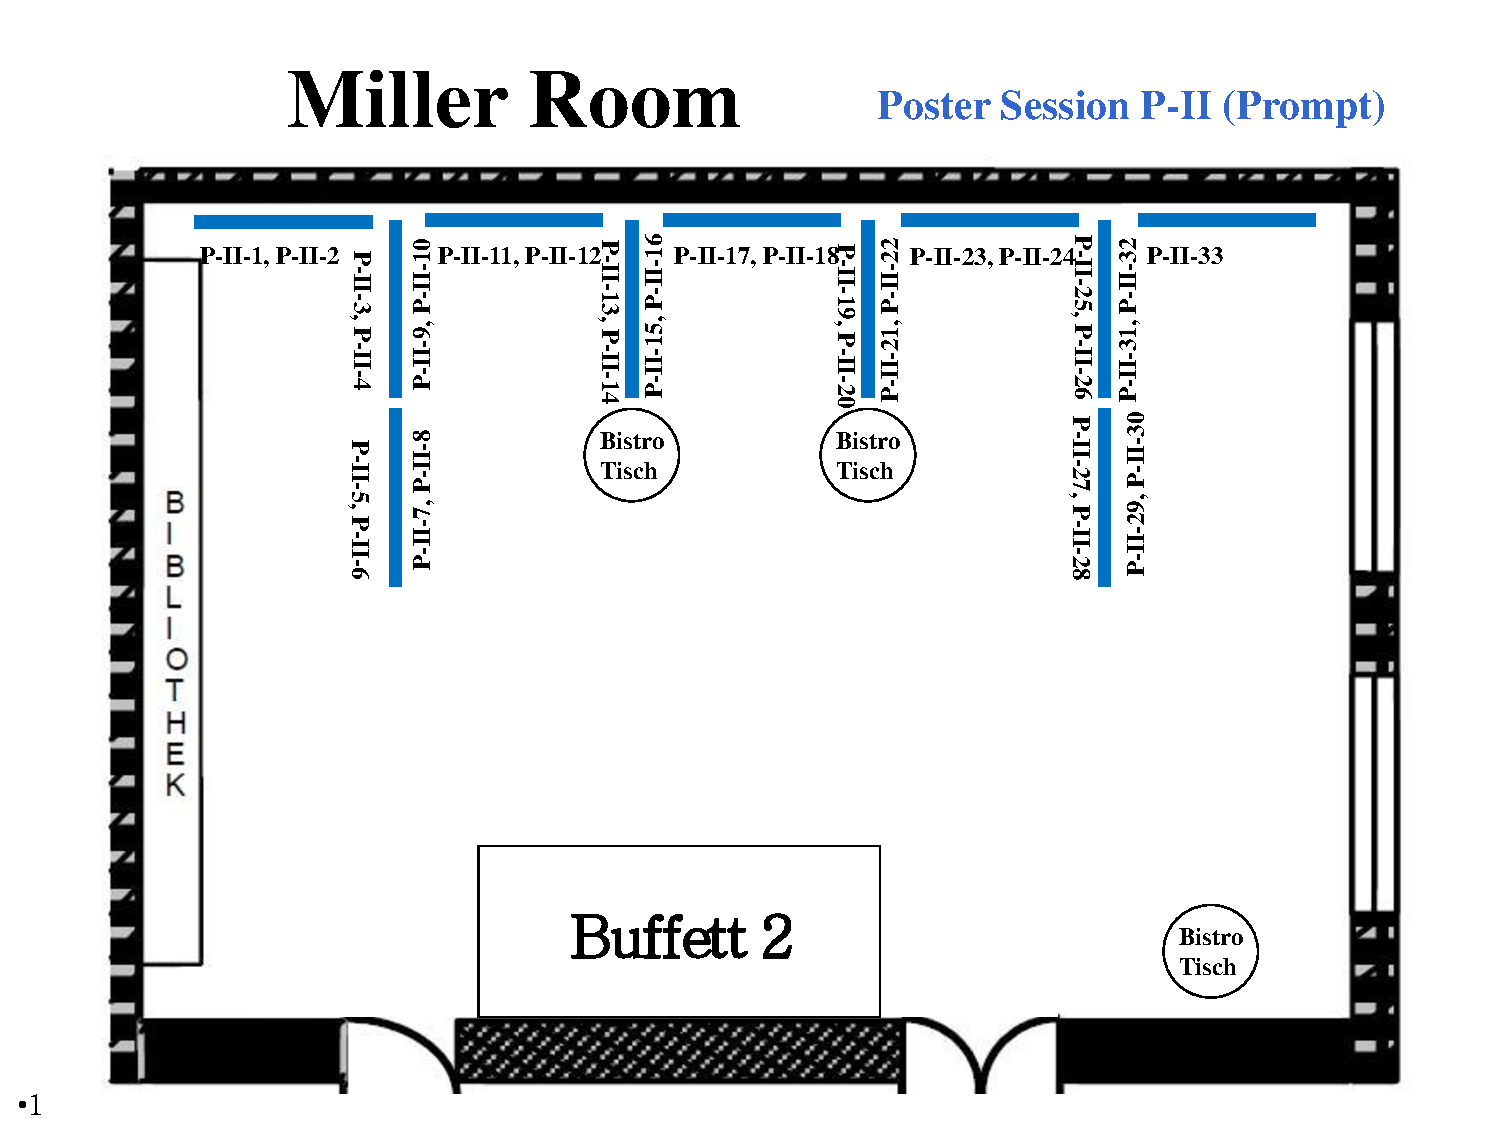
\includegraphics[scale=0.62,angle=90]{pg_0001.pdf}

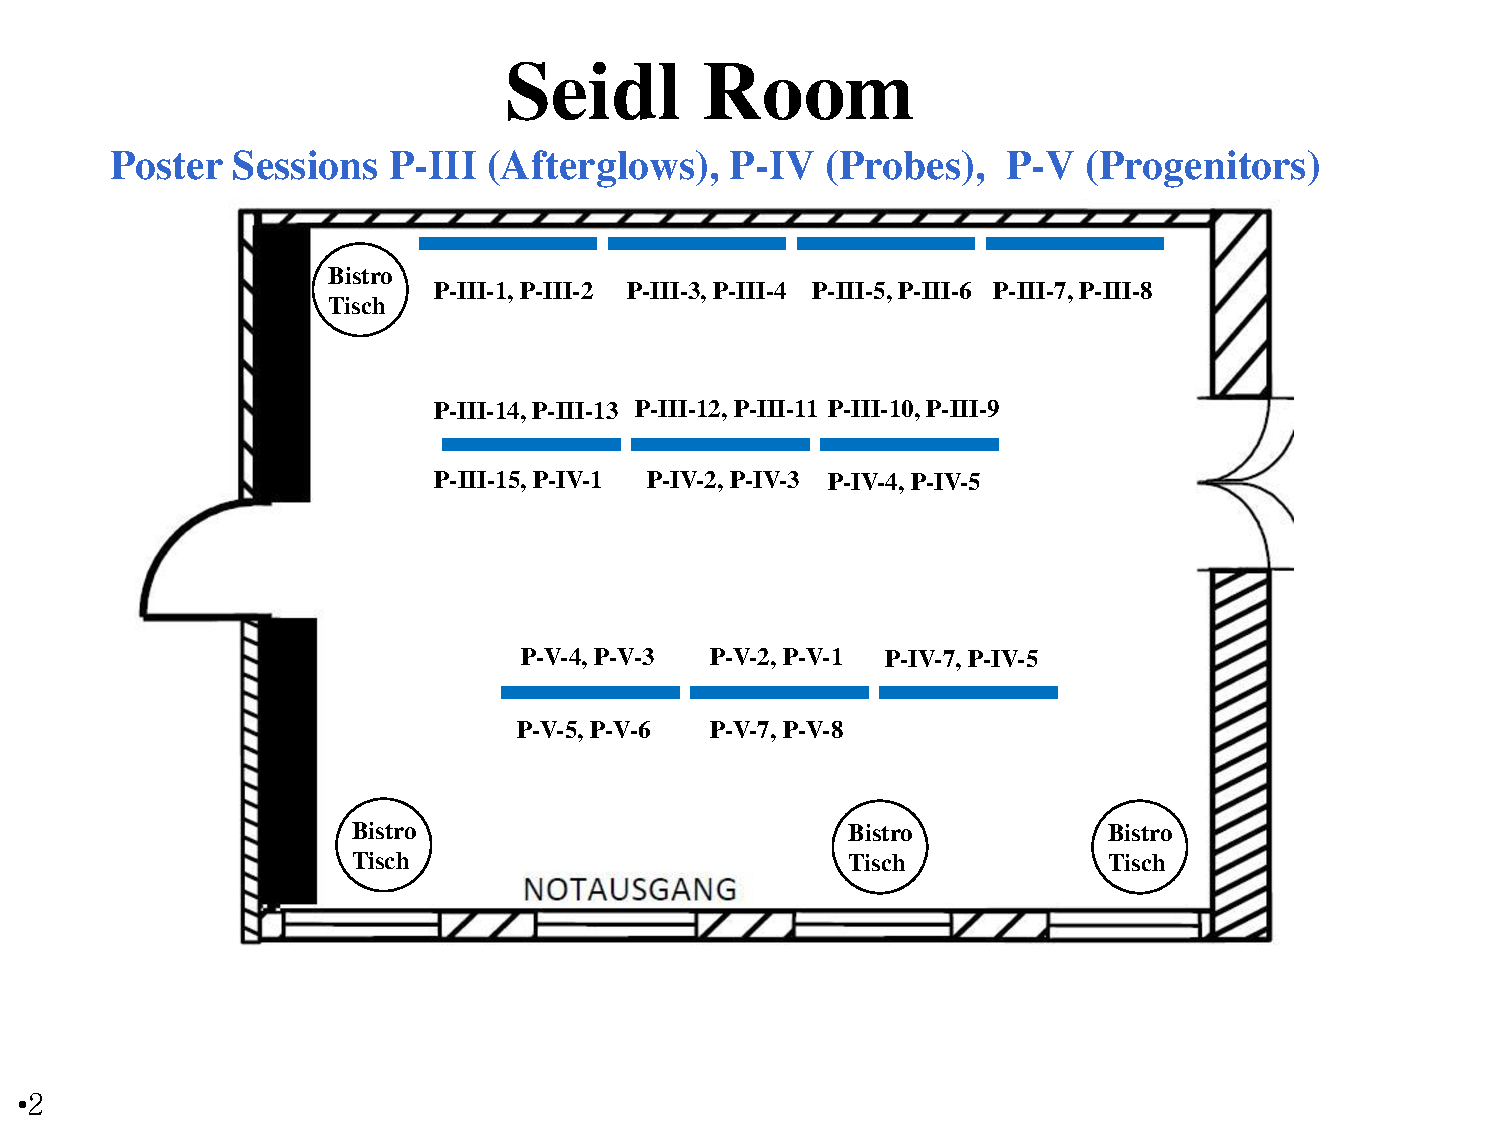
\includegraphics[scale=0.62,angle=90]{pg_0002.pdf}

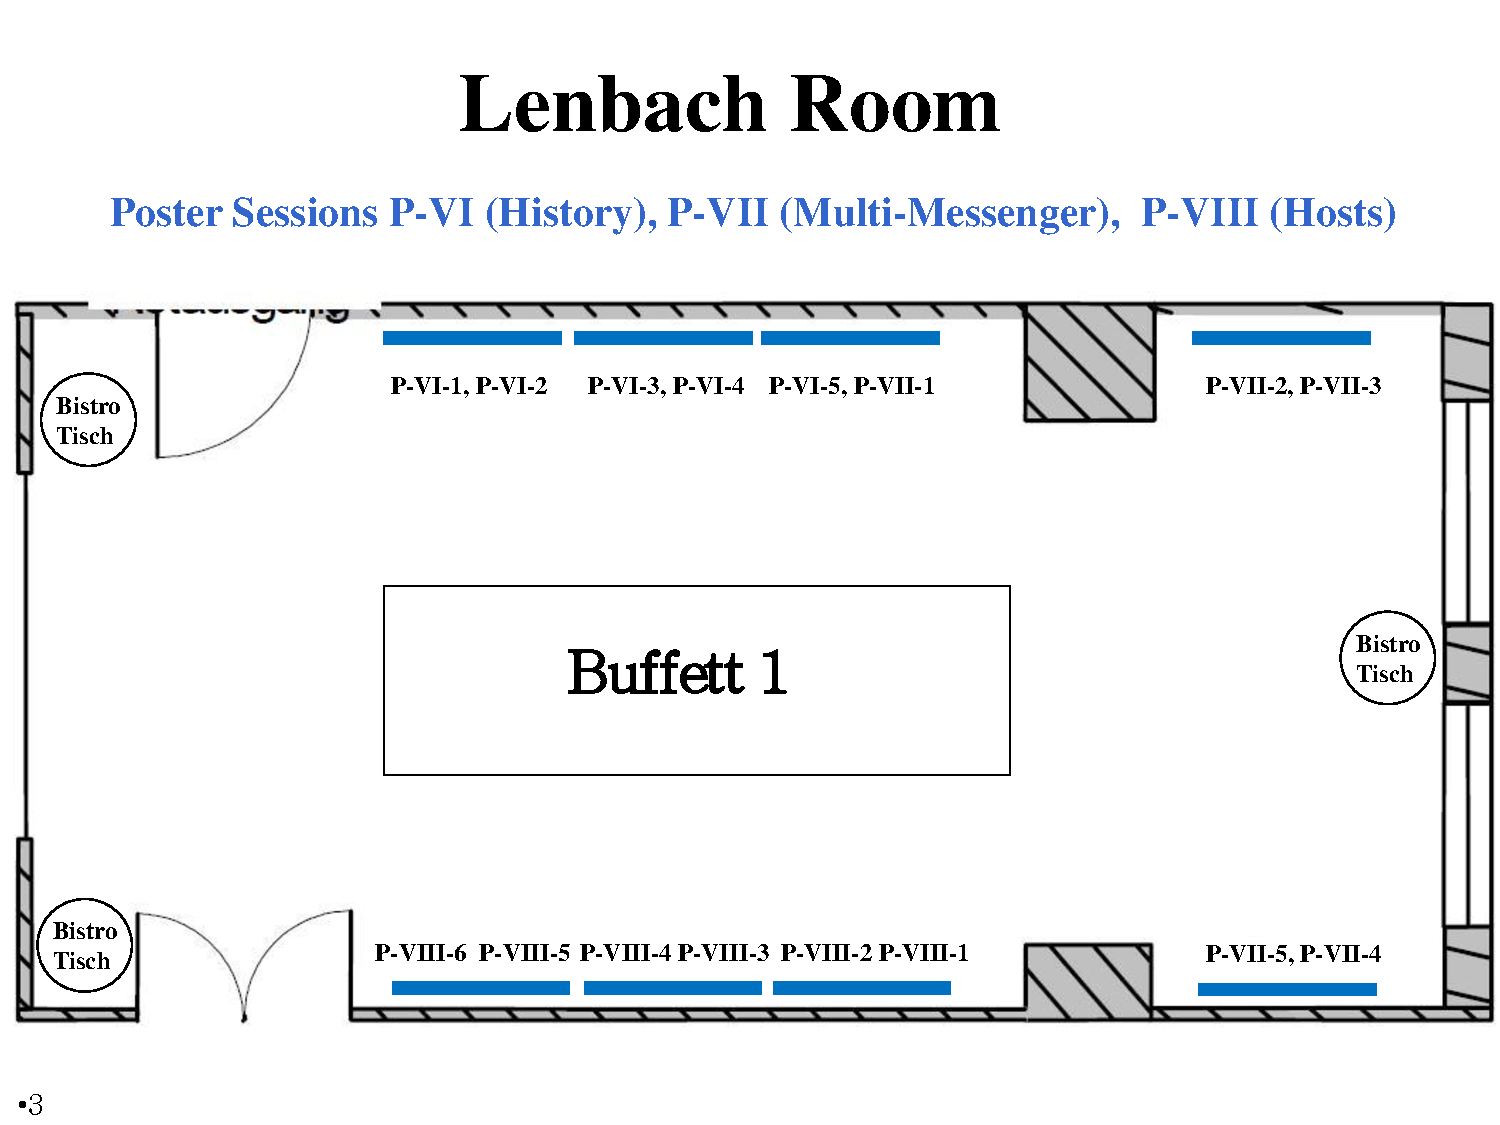
\includegraphics[scale=0.62,angle=90]{pg_0003.pdf}

\newpage

\redefineheaders{}{Index of Presenters}

\begin{center}
  \begin{longtable}{|p{1.6cm} |p{1.6cm} |p{2cm} |p{3cm} |}
    \hline
$IOP
    \hline
  \end{longtable}
\end{center}


\end{document}
